% Schematic view of a proton-proton collision producing HH -> bb tautau:
% hard process, initial- and final-state radiation, hadronization and underlying event.
% Compile with pdflatex; output included as figures/chapter_I/pp_event_sketch.pdf.
\documentclass[11pt,border=3pt]{standalone}
\usepackage[T1]{fontenc}
\usepackage{cochineal}
\usepackage[cochineal]{newtxmath}
\usepackage{tikz}
\usetikzlibrary{decorations.pathmorphing,decorations.markings,arrows.meta,calc,shapes.geometric}

% Okabe-Ito based palette
\definecolor{chard}{HTML}{D55E00}
\definecolor{crad}{HTML}{0072B2}
\definecolor{chad}{HTML}{009E73}
\definecolor{cue}{HTML}{CC79A7}
\definecolor{cprot}{HTML}{999999}

\tikzset{
  gluon/.style={decorate, decoration={coil, amplitude=1.6pt, segment length=3.2pt, aspect=0.6}, line width=0.6pt},
  quark/.style={line width=0.7pt},
  scal/.style={dashed, line width=0.8pt},
  lep/.style={line width=0.7pt, -{Stealth[length=4pt]}},
  hadron/.style={line width=0.5pt, -{Stealth[length=3pt]}, chad!80!black},
  cluster/.style={ellipse, draw=chad!70!black, fill=chad!25, minimum width=11pt, minimum height=7pt, inner sep=0pt},
  lab/.style={font=\footnotesize, inner sep=1.5pt},
}

% hadronization: a cluster at #1 oriented along angle #2, with three hadrons
\newcommand{\hadronize}[2]{%
  \node[cluster, rotate=#2] (h) at (#1) {};
  \draw[hadron] (h) -- ++(#2-22:0.55);
  \draw[hadron] (h) -- ++(#2:0.65);
  \draw[hadron] (h) -- ++(#2+22:0.55);
}

\begin{document}
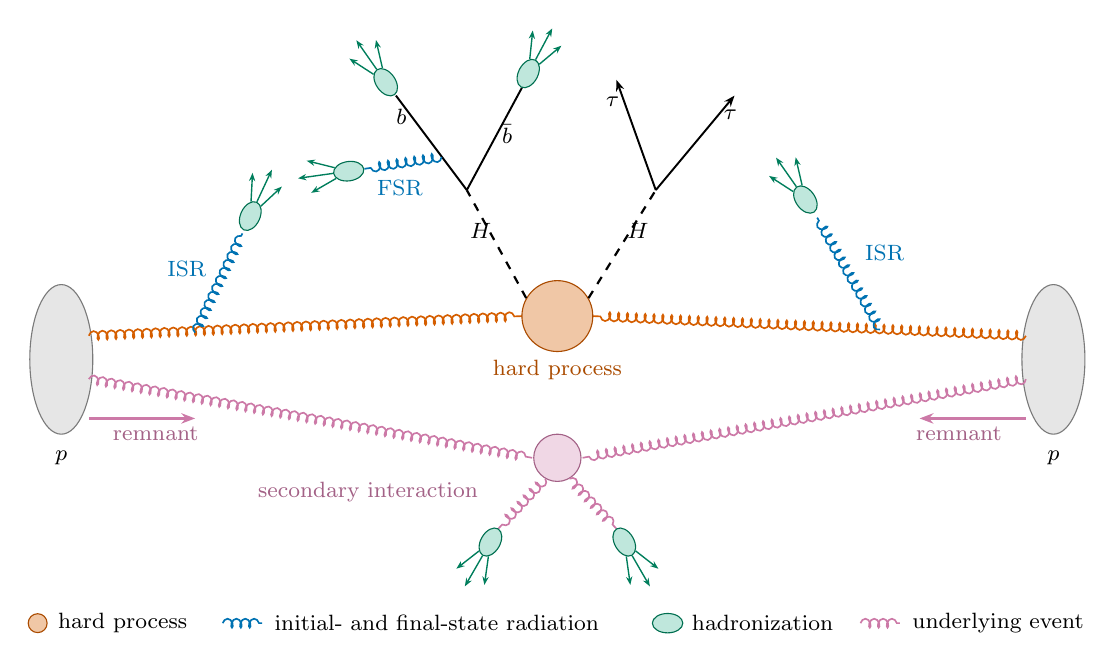
\begin{tikzpicture}[x=1cm,y=1cm]

  % ---------------- protons and remnants ----------------
  \node[ellipse, draw=cprot!80!black, fill=cprot!25, minimum width=0.8cm, minimum height=1.9cm] (pA) at (-6.3,0) {};
  \node[ellipse, draw=cprot!80!black, fill=cprot!25, minimum width=0.8cm, minimum height=1.9cm] (pB) at (6.3,0) {};
  \node[lab] at (-6.3,-1.25) {$p$};
  \node[lab] at (6.3,-1.25) {$p$};
  % beam remnants, continuing along the beam
  \draw[cue, line width=0.9pt, -{Stealth[length=5pt]}] (-5.95,-0.75) -- (-4.6,-0.75);
  \draw[cue, line width=0.9pt, -{Stealth[length=5pt]}] (5.95,-0.75) -- (4.6,-0.75);
  \node[lab, cue!80!black, anchor=north] at (-5.1,-0.8) {remnant};
  \node[lab, cue!80!black, anchor=north] at (5.1,-0.8) {remnant};

  % ---------------- hard process ----------------
  \coordinate (hp) at (0,0.55);
  \draw[gluon, chard] (-5.95,0.3) -- (-0.45,0.55);
  \draw[gluon, chard] (5.95,0.3) -- (0.45,0.55);
  \node[circle, draw=chard!80!black, fill=chard!35, minimum size=0.9cm] (hard) at (hp) {};
  \node[lab, chard!80!black, anchor=north] at (0,0.05) {hard process};

  % initial-state radiation
  \draw[gluon, crad] (-4.6,0.34) -- (-4.0,1.6);
  \draw[gluon, crad] (4.1,0.38) -- (3.3,1.8);
  \hadronize{-3.9,1.82}{65}
  \hadronize{3.15,2.03}{125}
  \node[lab, crad, anchor=east] at (-4.4,1.15) {ISR};
  \node[lab, crad, anchor=west] at (3.85,1.35) {ISR};

  % ---------------- H -> bb with final-state radiation ----------------
  \draw[scal] (hard.150) -- (-1.15,2.15) node[midway, lab, anchor=south east] {$H$};
  \draw[quark] (-1.15,2.15) -- (-2.05,3.35) node[pos=0.78, lab, anchor=east] {$b$};
  \draw[quark] (-1.15,2.15) -- (-0.45,3.45) node[pos=0.55, lab, anchor=west] {$\bar{b}$};
  \draw[gluon, crad] (-1.47,2.57) -- (-2.45,2.42);
  \node[lab, crad, anchor=north] at (-2.0,2.33) {FSR};
  \hadronize{-2.18,3.52}{125}
  \hadronize{-0.37,3.63}{62}
  \hadronize{-2.65,2.39}{188}

  % ---------------- H -> tautau (no QCD radiation) ----------------
  \draw[scal] (hard.30) -- (1.25,2.15) node[midway, lab, anchor=south west] {$H$};
  \draw[lep] (1.25,2.15) -- (0.75,3.55) node[pos=0.8, lab, anchor=east] {$\tau$};
  \draw[lep] (1.25,2.15) -- (2.25,3.35) node[pos=0.8, lab, anchor=west] {$\tau$};

  % ---------------- underlying event: secondary interaction ----------------
  \draw[gluon, cue] (-5.95,-0.25) -- (-0.32,-1.25);
  \draw[gluon, cue] (5.95,-0.25) -- (0.32,-1.25);
  \node[circle, draw=cue!80!black, fill=cue!30, minimum size=0.6cm] (mpi) at (0,-1.25) {};
  \draw[gluon, cue] (mpi.240) -- (-0.75,-2.15);
  \draw[gluon, cue] (mpi.300) -- (0.75,-2.15);
  \hadronize{-0.85,-2.32}{240}
  \hadronize{0.85,-2.32}{300}
  \node[lab, cue!80!black, anchor=north east] at (-0.95,-1.5) {secondary interaction};

  % ---------------- legend ----------------
  \begin{scope}[shift={(-6.6,-3.35)}]
    \fill[chard!35, draw=chard!80!black] (0,0) circle (0.12);
    \node[lab, anchor=west] at (0.2,0) {hard process};
    \draw[gluon, crad] (2.35,0) -- (2.85,0);
    \node[lab, anchor=west] at (2.95,0) {initial- and final-state radiation};
    \node[cluster] at (8.0,0) {};
    \node[lab, anchor=west] at (8.25,0) {hadronization};
    \draw[gluon, cue] (10.45,0) -- (10.95,0);
    \node[lab, anchor=west] at (11.05,0) {underlying event};
  \end{scope}
\end{tikzpicture}
\end{document}
